\chapter{稳定性}
\section{引言}
可靠性是所有器件设备都必须满足的一个主要指标,超导磁体当然不例外。历史上看,可靠性曾是超导磁体中最困难,因而也是最具挑战性的一个方面。
如图1.5所示,超导电性存在于由三个参数(电流密度$J$,磁场$H$和温度$T$)为边界的相体积内部。

这三个参数中的电流密度和磁场,至少在正常运行条件下,设计者是可以很好的定义并控制它们的。甚至在复杂的故障模式条件下,比如含有多个螺管的混合磁体或嵌套多线圈磁体,
电流密度和磁场也是可控的。可以说:磁体设计者能够牢牢掌控这两个参数。
到了温度参数,就不如此了。温度这三个参数中最难控的。相对运行点的温度偏移,在时间上难以预测,在空间上(即在线圈内部)就更难控制了。
储存在磁体内的磁场能和机械能,很容易转化为热能,引起线圈内部某些位置的导体温度上升到超过其临界值。
实际上,最终超导磁体的所有“稳定性问题”都可以归为磁体设计者不能控制线圈温度保持在运行点。

本章我们考虑 1)超导线圈内控制温度的基本物理问题;2)线圈内不可预测温升发生可能性的稳定性评估方法。
第7和第8章同样讨论不同条件下线圈内温升:第7章讨论温升的原因或源;第8章讨论控制磁体不可预测温升的保护方法。
首先,LTS和HTS磁体的稳定性问题就截然不同。

\textbf{LTS vs. HTS}

如图1.6给出的,稳定性的实现难度和费用随运行温度提高而降低。在下面的讨论中,我们将比较HTS和LTS的“稳定裕度”,并证明HTS磁体实际上
是非常稳定的。换句话说,任何HTS磁体都会达到其运行电流,且不会存在“提前失超(premature quench)”。
这种偶然事件仍经常影响“高性能”(即绝热和高电流密度)LTS磁体。
这意味着稳定性对于HTS磁体来说,不像在LTS磁体一样,是设计和运行中很严重的问题。
不过,稳定性仍然是HTS磁体的关键问题[6.1–6.8]。

\section{稳定性理论和标准}
我们从含温度$T$的单位超导体体积的功率密度方程出发,讨论载有额定电流$I_{op}$的磁体的热稳定性:
\begin{equation}
C_{cd}(T)\frac{\partial T}{\partial t}=\nabla ·[k_{cd}(T)\nabla T]+\rho_{cd}(T)J_{cd_o}^2(t)+g_d(t)-(\frac{f_p\ \mathrm{P_D}}{A_{cd}})g_q(T)
\end{equation}
式中,等式左侧导体热能密度的时间变化率,其中$C_{cd}(T)$是导体单位体积的热容。
这个公式是Stekly针对复合超导体,即由超导体和正常金属基底组成的超导体,提出的。
对于纯稳态稳定性,左侧项必须总为零;实际上,对大多数线圈,甚至对绝热线圈,
一个在运行温度$T_{op}$附近很小的温度漂移$\Delta T_{op}$都是允许的。
如前所述,因为HTS磁体允许的$\Delta T_{op}$通常远大于LTS磁体,稳定性对HTS磁体来说,
几乎不成问题。这一点下面将更详细的阐述。

等号右侧的各项均为单位体积值。第一项是通过热传导进入复合导体的热量,式中$k_{cd}(T)$是复合导体的热导率。
第二项是焦耳热,式中$\rho_{cd}(T)$是复合导体的电阻率(在超导态为零),$J_{cd_o}(t)$是运行电流$I_{op}(t)$
下的依赖于时间的电流密度。$g_d(t)$给出的是主要由磁和机械效应产生的非焦耳热。最后一项表示冷却,其中$f_p$
是复合导体与制冷机接触的湿润周长$\mathcal{P}_D$分数,$A_{cd}$是复合导体截面积,$g_d(T)$是与制冷剂
之间的对流热流。

稳定性(以及第8章将要讨论的保护)理论和概念的发展史就是对方程6.1简化求解的历史。
表6.1列出了由方程6.1在特定工况下导出的概念。
表中,标为0的参数表示它在方程中可以忽略或者不予考虑。$\surd$表示要予以考虑。
在讨论方程6.1的每一项之前,我们先简要讨论表6.1中列出的概念。

表格6.1

\subsection{公式6.1涉及的概念}
下面将简要讨论方程6.1所涉及的以及表6.1列出的概念。
\begin{description}
  \item[磁通跳跃] 第五章已经考察得到了避免通常会影响LTS的多数磁通跳跃的准则。
  \item[低温稳定性] 低温稳定性的基本概念是在1960年代中期作为实现磁体可靠运行的工程方案而提出的[6.9]。
  在一个低温稳定的复合导体中,超导体与高导电基底金属同步处理[6.10],导体的大部分表面与制冷工质接触以
  保证“局域”冷却。如表6.1所给出的,除了焦耳热项和冷却项,其他项可以忽略。1970年代很多成功的磁体都是
  低温稳定的[6.11, 6.12];当前,它仅用于``大型``LTS磁体。稍后我们将看到,它并不用于HTS磁体。
  低温稳定的概念将在本章的专题中进一步研究。
  \item[动态稳定性] 第五章研究过第II类超导体中当磁扩散远大于热扩散时,若导体的尺度(如带材)不足以抑制它,
  将发生磁通跳跃。通过将超导体和高热导率材料,比如铜,复合,我们可以平衡这两种扩散效应,实现无磁通跳跃
  的稳定运行。LTS带材如今已很少使用;磁通跳跃也和HTS带材不一样(讨论5.7)。所以,后文将不再讨论这个准则。
  \item[等效面积] ``等效面积``准则是低温稳定性的特例,即包含了方程6.1中的热传导项$\Delta\cdot[k_{cd}(T)\Delta T]$。
  这样,可以提高低温稳定磁体的总体电流密度。本准则将在专题中进一步讨论。
  \item[MPZ] 最小传播区域(minimum propagating zone, MPZ)的概念考虑在绕组中施加局域扰动$g_d(t)$对
  线圈性能的影响[6.13]。MPZ概念表明,即使在绕组中存在少量的正常态区域,磁体仍可能保持超导态,当然前提是
  正常态区域体积小于MPZ理论定义的临界尺度。它在绝热磁体中的重要性首先被Wilson在1970年代末期注意到[1.27],
  此后,它成为分析绝热磁体稳定性不可或缺的概念。MPZ概念将在专题中进一步研究。  
  \item[不稳定情况] 表6.1中最后两种情况涉及非稳定态的绕组热行为。第8章将讨论。
\end{description}

\subsection{热能}
长期稳定性要求$\partial T/\partial t\simeq 0$;对于给定的热输入,它反比于$C_{cd}(T)$,在超导磁体
可能运行温区2--90 K内有数量级的变化。
表6.2给出了由第四章讨论过的冷却方式冷却的超导磁体的绕组材料
NbTi、$\mathrm{MgB_2}$、YBCO以及附属材料在相应温区内的近似热容。

表中,NbTi、$\mathrm{MgB_2}$和YBCO的运行温区分别设定为2--10 K、2--30 K、2--90 K。
对稳定性而言,影响最大的材料是铜(它用以代表正常电导的基底金属;其他还包括铝和银)和超导体本身。
因为铜在10--20 K区间($\mathrm{MgB_2}$的区间类似)的$C_p(T)$比在2--4 K区间大好几个数量级,
在50--90 K区间(YBCO)又会高出几个数量级,所以这就很明确的告诉我们:就稳定性而言,最好的是YBCO,
其次是$\mathrm{MgB_2}$,对磁体工程师的挑战是最小的。
我们的结论是,只有对于LTS,稳定性才真正算作问题。

表格6.2

\subsection{热传导}
在低温稳定性中,热传导项被略掉。而在“绝热”LTS磁体中,它对决定MPZ大小有重要的作用;MPZ大小反过来
决定了绝热绕组可以允许的“局部”扰动的程度。
本章的专题中,我们将会研究发现,这一项还决定了制冷机冷却的绝热磁体的绕组可承受的以限制最大温升的
稳态耗散能量密度(即交流损耗)水平。
表6.3与表6.2类似,给出了热导率$k(T)$的近似值。

表格6.3

和热容不同,表中每一种材料的热导率随温度变化的幅度并不剧烈。
铜有最好的热导率,比其他材料好很多。这让它成为LTS和HTS绕组稳定(本章)和保护(第8章)不可或缺的首选材料。
第七章将会讨论,由于铜绕组在时变电磁场下的涡流焦耳耗散,使用铜可能造成运行上的困难,所以复合超导体一般通过
复杂的配置尽量避免或减少铜的影响。

\subsection{焦耳热}
在正常运行条件下,超导磁体的焦耳热项是0。因为第II类超导体(除了Ni)基本都是元素合金或化合物,
第II类超导体的正常态的电阻率一般远大于铜等基底金属的电阻率。
这一点已在讨论5.5中(磁场和热扩散)研究了。
Stekly的稳定性理论的一个要点是:当超导体不超导后,用高导电性的正常金属旁路掉高电阻的超导通路。
(另一个是提供足够的冷量移除此焦耳热)
表6.3同时列出了铜和不锈钢的电阻率$\rho(T)$,它可用于近似正常态的超导体。但如随后的专题所将讨论的,
当临界电流附近的磁通流效应必须考虑的时候,上述近似不可用。

\subsection{扰动谱}
方程6.1中的$g_d(t)$项代表的是绕组内部可引起温升的除了焦耳热的所谓扰动或热流密度。
扰动可以同时从时间和空间的角度来刻画,时间上可以是短时的(由能量给出的扰动)也可以是连续的(有功率给出);
空间上可以是局域的(能量或功率)也可以是全局的(能量密度或功率密度)。
突然的导体滑移---导线运动---是一个很好的短时、局域扰动的例子,可以很好的用滑移向绕组内释放的总能量来定量
刻画。或许最好的连续、全局的扰动例子是交流损耗,它是持续将能量释放到交流设备绕组中的。
置于连续和全局热流密度中的绝热绕组的一个设计事项将在专题中研究。

图6.1给出了LTS磁体多年来总结汇集的六种主要扰动源的扰动谱[6.14]。
这些源中,磁通跳跃、导线运动和交流损耗是“内秉的”,因为他们产生于绕组之内;
漏热与绕组和外部的耦合有关;粒子洒落和原子核热与特定的器件有关,在多数磁体中可以忽略。

如第五章讨论的,磁通跳跃对LTS,特别是对HTS现在可以视为有利的。
导线运动和其他机械事件会影响绝热LTS磁体。
然而,甚至绝热HTS磁体通常也都不会受到这些扰动的影响。
因为第II类超导体在时变电磁场下有耗散,这令HTS和LTS在交流损耗下同样脆弱。
对交流损耗最小化的程度毫无疑问将促成或阻止HTS在电力上的广泛应用。

\begin{figure}[htbp]
	\centering
	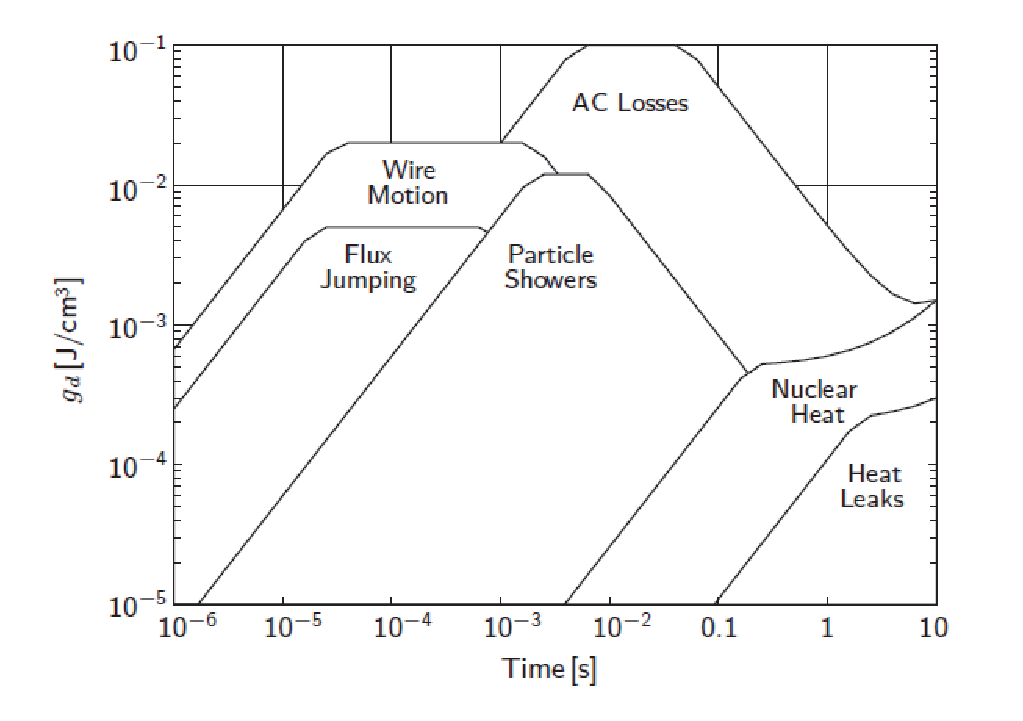
\includegraphics[scale=0.6]{chpt6/figs/fig6.1.eps}
	\caption{汇集的$g_d(t)$谱。}
\end{figure}

\subsection{稳定裕度 vs 扰动能}
所谓的“稳定裕度”或简单的“能量裕度”对绝热超导磁体是尤其有用的设计参数。
它就是载有运行电流$I_{op}(I_t)$的冷却或绝热的复合超导体所能吸收而又能维持全超导的
最大能量密度$\Delta e_h$。除非冷量可以平衡这个$\Delta e_h$,否则复合超导体将被加热,
其温度降上升至运行温度$T_{op}$之上;当它继续加热超导与$I_{op}$有关的“分享电流”温度$T_{cs}(I_{op})$
后,失去全超导。图6.2给出了第II类超导体临界电流与温度的关系$I_c(T)$,其中定义了$T_{cs}(I_{op})$。
$I_c(T)$近似是一条直线,连接了$T_{op}$下的临界电流$T_c(T_{op})\equiv I_{c_o}$以及$I_c(T_c)=0$。
实心原点定义$T_{cs}(I_{op})$为$I_c(T)$线和$I_{op}$对应的虚线的交点。
注意到$T_{cs}(I_{op})$是载有$I_{op}$的复合导体甚至在绝热条件下可以保持全超导的最高温度。
超过$T_{cs}(I_{op})$,基底常导金属开始“分享”电流,产生焦耳热耗散。
在绝热线圈中,从$T_{cs}(I_{op})$到临界温度$T_c$的转变差不多是瞬时的,在$T_c$及以上问题下,
基底材料载有差不多全部电流。
在图中还定义了$[\Delta T_{op}(I_{op})]_{st}=T_{cs}(I_{op})-T_{op}$,即复合导体从$T_{op}$
往上还能保持全超导所能承受的最大温度漂移极限。
有时候使用$[\Delta T_{op}(I_{op})]_{st}$而不是$\Delta e_h$来定量表示稳定性的程度。
在绝热条件下,$\Delta e_h$表示为: 
\begin{equation}% page357 第1个
\Delta e_h=\int_{T_{op}}^{T_{cs}(I_{op})}{C_{cd}(T)d(T)}=\int_{T_{op}}^{T_{op}+[\Delta T_{op}(I_{op})]_{st}}{C_{cd}(T)d(T)}
\end{equation}
注意到,$\Delta e_h$不仅依赖于$C_{cd}(T),T_{op}$和$T_{cs}(I_{op})$或$[\Delta T_{op}(I_{op})]_{st}$,
还依赖于与$I_{c_o}$有关的$I_{op}$($i_{op}\equiv I_{op}/I_{c_o}$)。
特别的,对于如图6.2这样的对$I_c(T)$的简单直线近似,$[\Delta T_{op}(I_{op})]_{st}$可由下式给出:
\begin{equation}% page357 第2个
[\Delta T_{op}(I_{op})]_{st}=(T_c-T_{op})(1-i_{op})
\end{equation}
\begin{figure}[htbp]
	\centering
	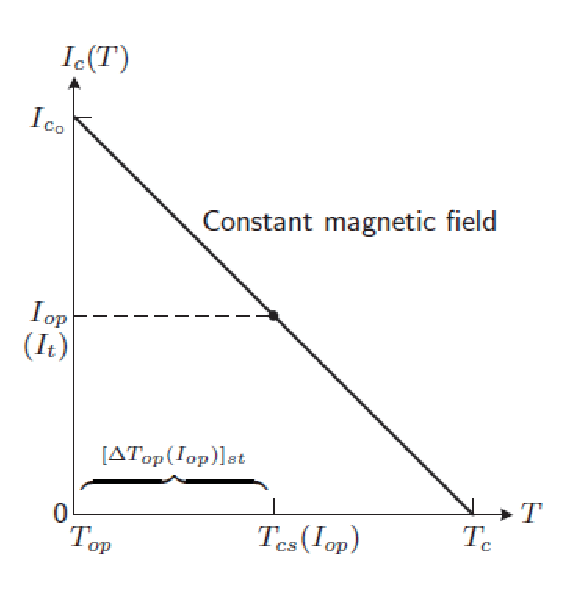
\includegraphics[scale=0.6]{chpt6/figs/fig6.2.eps}
	\caption{某第II类超导体的$I_c(T)$直线近似。}
\end{figure}
从方程6.3,我们可以得出,对一个绝热磁体,它的电流分享温度必须大于其运行温度($T_{cs}>T_{op}$),也即
它的$I_{op}(I_t)$应当在绕组中低于导体的最小$I_{c_o}$。因为$I_{c_o}$与磁场有关,而磁场在绕组中是变化的。
表6.4列出了几个对LTS和HTS磁体比较典型的$T_{op}$和$\Delta T_{op}$及其对应的$\Delta e_h$。

表6.4.。。。。。

\begin{description}
	\item[LTS] 对比表6.4中给出的能量裕度与图6.1中给出的扰动能量密度,可以明确看到,LTS磁体非常容易因扰动
	而失超,失超对应的能量密度由方程6.1中的$g_d(t)$表示。为了应对这个情况,多年来人们一直进行技术开发以
	抑制这些扰动,如导线运动、磁通跳跃。对多数“直流”LTS绝热磁体,要最小化交流损耗以使其在大部分时间稳定运行。
	最小化或消除机械扰动(如导线运动)的技术仅对LTS磁体比较重要,第七章简要讨论。
	\item[HTS] 除了交流损耗,HTS磁体的扰动能量谱如图6.1所示。根据表6.4中的$\Delta e_h$,我们可以得出,HTS
	磁体至少在DC条件下,是绝对稳定的:于是,每一个DC HTS磁体都应被设计为绝热运行的。
\end{description}

\subsection{冷却}
尽管每一个超导磁体的运行都需要冷却,但如第四章论及,仅浸泡式低温稳定磁体需要\emph{在绕组间}用制冷剂冷却。
这样,方程6.1中的$-g_q(T)$项仅用于表示绕组内的冷却;绕组外的冷却,是每一个超导体都要求的,一般而言是外沿的;
它不出现于方程6.1中。
如上文讨论,HTS磁体能够,实际上也总是,绝热运行。此外,除了因耦合LTS磁体而运行于液氦温区的,多数HTS磁体都是
在$\sim$20 K以上运行。所以,液氦的传热数据对浸泡低温稳定HTS磁体设计不再是非常重要的;甚至液氮的传热数据
对HTS磁体也不是非常重要的,这是因为绝热运行时,绕组中根本没有液氮。

Bottura总结了氦在不同冷却区间的传热系数$h_q$与$\Delta T$的关系,如图6.3[6.14];这里的$\Delta T$一般是指
加热表面和4.2 K氦之间的温差。图中包括:1)核态沸腾和膜态沸腾,包括核态沸腾峰值点$h_{pk}=1.23\ \mathrm{W/cm^2 K}$;
2)暂态核沸腾;3)1.8 K(超流)和4.2 K下的Kapitza;4)3.5 atm和4.5 K下$10^4$和$10^5$两个雷诺数下的迫流。
这些图线中,包含峰值点的核态沸腾图是由浸泡式低温稳定磁体得出的;1.8 K的Kapitza图针对的是超流氦冷却的低温稳定磁体;
迫流图是针对的CICC绕成的低温稳定磁体。
\begin{figure}[htbp]
	\centering
	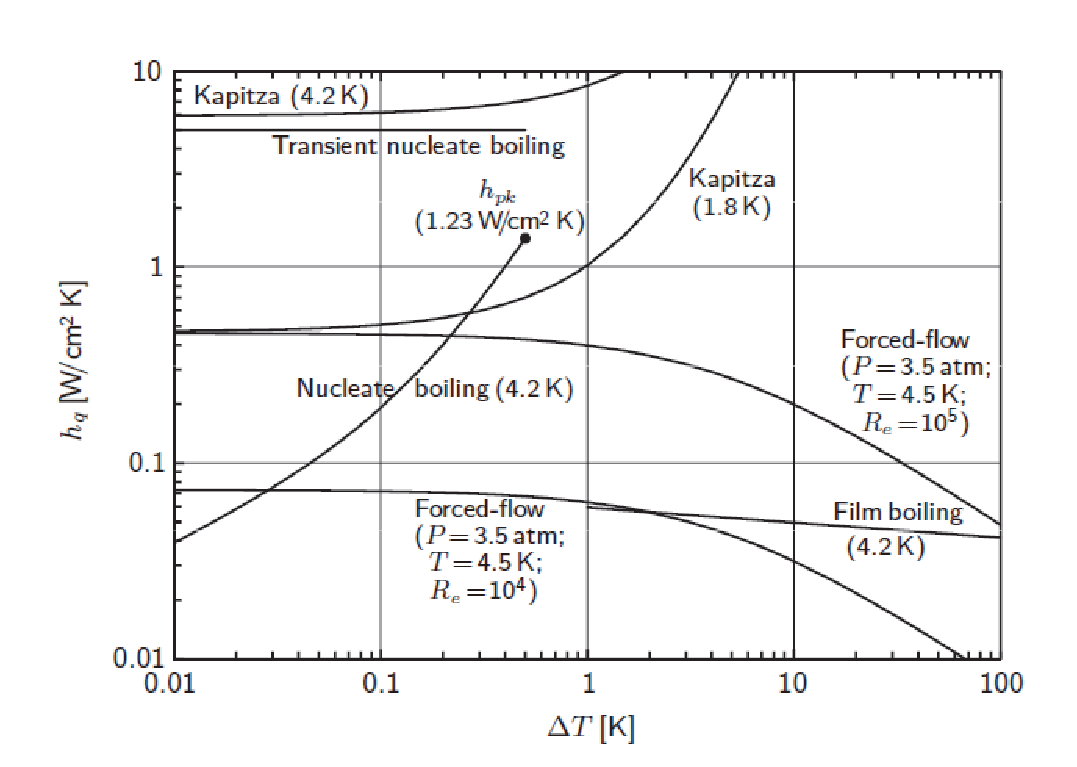
\includegraphics[scale=0.6]{chpt6/figs/fig6.3.eps}
	\caption{传热系数$h_q$与$\Delta T$的关系。}
\end{figure}

\section{电流密度}
磁体产生的磁场的计算中,一个关键参数是总电流密度$\lambda J$(方程3.108),它是由总安匝数$NI$除以磁体绕组截面积,
截面不仅包括载流导体,同时也包括绕组中的非载流部分。图6.4(a)给出了复合导体的截面积组成部分,图6.4(b)定义了整个
绕组的组成部分。两个图给出的是各部件代表性的常用组分。
\begin{figure}[htbp]
	\centering
	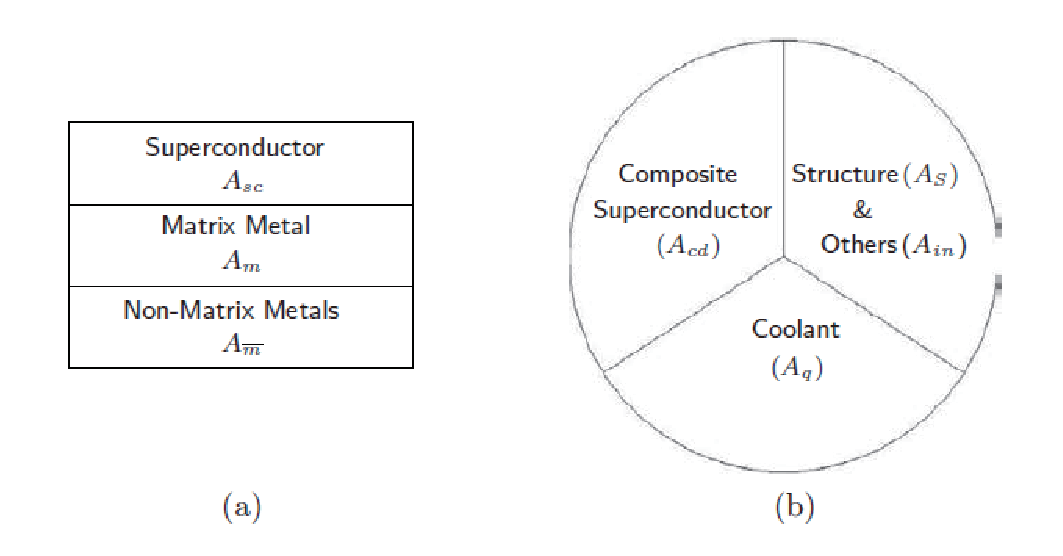
\includegraphics[scale=0.6]{chpt6/figs/fig6.4.eps}
	\caption{截面积的示意图:(a)复合导体;(b)全绕组。}
\end{figure}
\subsection{截面积}
如图6.4所示,超导体中至少有7个不同的截面积用于定义不同的电流密度:
图6.4a中对复合导体有$A_{sc},A_m$和$A_{\bar{m}}$;图6.4b中对全绕组有$A_{cd},A_s,A_{in}$和$A_q$。
$A_{\bar{m}}$,是非基底金属,在NbTi等合金中是0,但在$\mathrm{Nb_3 Sn}$和YBCO等化合物导体中不可忽略。
注意到,其他材料如绝缘体等占据的截面并未包括到总的超导体截面中来。
$A_S$通常是金属加强材料占据的截面,$A_{in}$包括绝缘体和有机填充材料如环氧等占据的截面。
除了下面将讨论的CICC导体,$A_S$和$A_{in}$通常可以统一归为结构部件。
复合导体和全绕组的总的截面积为:
\begin{subequations}
	\begin{align}
	A_{cd}&=A_{cs}+A_m+A_{\bar{m}}\\
	A_{wd}&=A_{cd}+A_S+A_{in}+A_q
	\end{align}
\end{subequations}

\subsection{复合超导体}
下面将定义并描述复合超导体的三个常用电流密度。

\textbf{超导体临界电流密度}

超导体临界电流密度$J_c$是由超导体在一定温度和磁场下的临界电流$I_c$除以截面$A_{sc}$(对NbTi和YBCO这种$A_{sc}$
可以明确量化的材料)或者$A_{sc}+A_{\bar(m)}$(对$\mathrm{Nb_3 sN}$这样非基底金属是一个联合部分的材料)得到的:
\begin{subequations}
	\begin{align}
	J_c&\equiv\frac{I_c}{A_{sc}}\\
	J_c&\equiv\frac{I_c}{A_{sc}+A_{\bar{m}}}
	\end{align}
\end{subequations}
在材料发展阶段中(表1.4中的阶段1),定义为$J_c\equiv I_c/A{sc}$的$J_c$以及$H_{c2}$和$T_c$是描绘超导体性能
的最合适、最有用的参数。

\textbf{工程(或导体)临界\& 运行电流密度}

工程(或导体)临界\& 运行电流密度$J_e (J_{cd})$考虑了工艺和磁体需求。$A_{\bar{m}}$和$A_m$都是磁体级别超导体
的关键参数:
\begin{equation}% page360 第5个
J_e=J_{cd}\equiv\frac{I_c}{A_{cd}}=\frac{I_c}{A_{sc}+A_m+A_{\bar{m}}}
\end{equation}
在CICC导体(讨论6.6)中,结构组分$A_S$和制冷工质组分$A_q$的截面也是导体的组成部分,所以他们也常被包含到$A_{cd}$
中去。当导体运行于电流$I_{op}$时,我们还可以定义工程(或导体)运行电流密度:$J_{e_o}=J_{cd_o}\equiv I_{op}/A_{cd}$。
$J_{cd_o}(t)$隐含了$I_{op}(t)$可随时间变化。

\textbf{基底电流密度}

基底电流密度$J_m$对由复合导体绕成的磁体的稳定性和保护是一个非常重要的参数。$J_m$定义为通过基底的电流除以其截面积。
\begin{equation}% page361 第1个
J_{m}\equiv\frac{I_m}{A_m}    \ \mbox{or}\    J_m(t)\equiv\frac{I_m(t)}{A_m}
\end{equation}
其中,$I_m$是运行(传输)电流$I_{op}(I_t)$的一部分或全部,而$I_{op}(I_t)$取决于超导体是否超导。
\begin{align*}% page361 第2个
I_{op}=I_t=I_m+I_s  \ \mbox{or}\ I_{op}(t)=I_{t}(t)=I_m(t)+I_s(t) \tag{6.7b}
\end{align*}
式中,$I_s$是通过超导体的电流。因为最相关的基底电流就是正常运行电流$I_{op}$,所以当$I_s=0$时,
常用另一个基于$I_{op}$的基底电流密度:
\begin{align*}% page361 第3个
J_{m_o}\equiv I_{op}   \ \mbox{or}\  J_{m_o}(t)\equiv\frac{I_{op}(t)}{A_m} \tag{6.7c}
\end{align*}

\subsection{绕组中的电流密度}
由第三章的研究以及上面简要的概述,我们知道磁体产生的磁场直接正比于磁体绕组的全电流密度。
我们可以使用两个电流定义这个电流,一个是表示任意电流的$I$,另一个是表示磁体运行电流的$I_{op}$:
\begin{subequations}
	\begin{align}
	\lambda J&\equiv\frac{I}{A_{wd}}\\
	\lambda J_{op}\equiv\frac{I_op}{A_{wd}}&  \ \mbox{or}\  \lambda J_{op}(t)\equiv\frac{I_{op}(t)}{A_{wd}}
	\end{align}
\end{subequations}
因为在这里讨论的所有电流密度中,是$\lambda J_{op}$决定了磁体产生的场,所以它对磁体费用的影响最为直接。
因此,对一个在市场中有竞争力的磁体而言,$\lambda J_{op}$必须尽可能的大,当然也需要考虑具体的磁体的设计、运行需要。
(第三章中,为了简单起见,$\lambda J_{op}$由$\lambda J$取代了。)

\textbf{CICC导体的电流密度}

CICC导体,用于大型和高场磁体(将在讨论6.6详细描述)。
因为在CICC中,导体和绕组是耦合的,我们需要特别定义一个导体电流密度$J_{cic_o}$,描述运行电流下的CICC导体:
\begin{subequations}
	\begin{align}
	J_{cic_o}\equiv\frac{I_{op}}{A_{cic}}\ \mbox{or}\ J_{cic_o}\equiv\frac{I_{op}(t)}{A_{cic}}\\
	A_{cic}\equiv A_{cd}+A_S+A_q
	\end{align}
\end{subequations}


\section{专题}
\subsection{讨论6.1:低温稳定性——电路模型}
此处我们讨论低温稳定性的理论。我们采用电路模型来研究由超导体嵌入铜基底而组成的复合导体的行为。

图6.5a给出了超导体的理想$R_s$和$I$关系图,其中,$R_s$是超导体的电阻---这个图可用于多数LTS,
而对多数HTS不适用。此处所谓的理想,是指在$I_s<I_c$时,$R_s=0$,其中$I_c$是超导体的临界电流。
在$I_s>I_c$时,$R_s=R_n$,其中,$R_n$是超导体在正常态的电阻;在$I_s=I_c$时,$0\le R_s\le 	R_n$,
也即它满足电路条件。图6.5b给出了在温度$T$下载有传输电流$I_t$的复合超导体的电路模型。
$I_s$是通过超导体的电流,$R_m$是基底金属的电阻;一般有$R_m\ll R_n$。

\textbf{$I_t\le I_c$区}\quad 此时,超导体载有全部传输电流,$I_s=I_t\le I_c$。由图6.5a有$R_s=0$,
由图6.5b有$V_{cd}=0$,其中$V_{cd}$是复合导体上的电压。总焦耳热耗散$G_j$为零。

\textbf{$I_t>I_c$区}\quad 当$I_t>I_c$,由于$R_m\ll R_n$,超过$I_c$的电流几乎都将流过铜基底。
也即。$I_m\simeq I_t-I_c$以及$I_s\simeq I_c$。其中,$I_m$是通过基底的电流。于是:
\begin{subequations}
	\begin{align}
	V_{cd}&=R_mI_m\simeq R_m{(I_t-Ic)}\\
	G_{j}&=V_{cd}I_t
	\end{align}
\end{subequations}
联立上面两个方程,有:
\begin{equation}% page362 第3个 6.11
{(G_j)}\simeq R_{m}I_{t}{(I_t-I_c)}
\end{equation}
注意,$G_j$与温度无关,和$R_m,I_c$一样。因为基底金属(如铜)的电阻在4-30 K范围内几乎与温度无关,
$R_m$在LTS的稳定性分析时,总是假定为常数。
\begin{figure}[htbp]
	\centering
	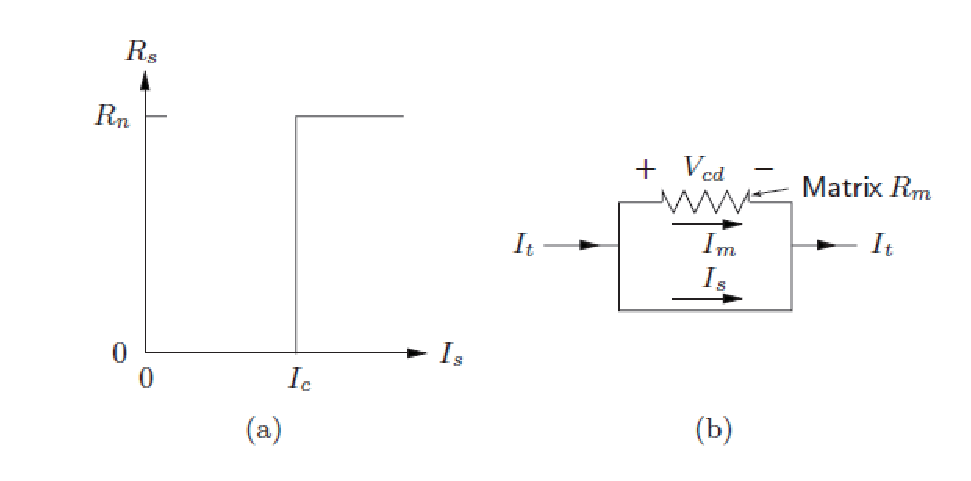
\includegraphics[scale=0.6]{chpt6/figs/fig6.5.eps}
	\caption{(a)超导细丝$R_s$和$I$关系图;(b)复合超导体的电路模型。}
\end{figure}

\subsection{问题6.1:低温稳定性——温度依赖}
下面我们考察复合导体单位长度总焦耳热耗散$G_j$对温度的依赖关系(讨论6.1中的方程6.11)。
图6.6(与图6.2相同)给出了$I_c$与$T$的关系,该关系常用于近似超导体在恒定磁场下的$I_c(T)$
(方程5.38给出了临界电流密度的相同的线性近似)。
注意到$I_c(T_{op})=I_{c_o},\ I_c(T_c)=0$。当温度变化时,通过复合导体的净传输电流$I_t$仍保持不变。
电流分享温度$T_{cs}$如图,有$I_t=I_c(T_{cs})$给出。

a) 超导体的$I_c(T)$由下式近似:
\begin{equation}% page363 第1个 6.12
I_c(T)=I_{c_o}(\frac{T_c-T}{T_c-T_{o_p}}) (T_{o_p}\leq T \leq T_c)
\end{equation}
证明,$G_j$有如下的温度依赖关系:
\begin{subequations}
	\begin{align}
	G_j(T)&=0 &(T_{o_p}\leq T \leq T_{cs})\\
	G_j(T)&=R_mI_t^2(\frac{T-T_{cs}}{T_c-T_{cs}})&(T_{cs}\leq T\leq T_c)\\
	G_j(T)&=R_mI_t^2 &(T\ge T_c)
	\end{align}
\end{subequations}
假定$R_m$与温度无关。

b) 画出从$T_{op}$到$T>T_c$温度范围的方程6.13的关系图。

c) 给出方程6.13b给出的$G_j$的物理解释。

d) 定性的讨论方程6.13b如何在30 K以上修正。30 K之上,$R_m$将依赖于温度,成为$R_m(T)$,这是复合HTS的情况。

\begin{figure}[htbp]
	\centering
	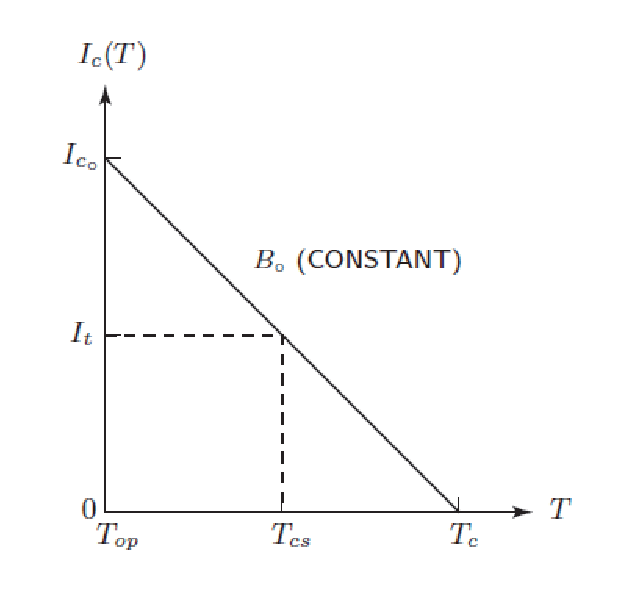
\includegraphics[scale=0.6]{chpt6/figs/fig6.6.eps}
	\caption{超导体的$I_c(T)$线性近似。}
\end{figure}

\subsubsection{问题6.1之解}
a) 因为$T_{op}\le T\le T_{cs}$时,有$I_c(T)>I_t$(图6.6),我们有:
\begin{align*}
G_j(T)=0 \quad (T_{o_p}\leq T \leq T_{cs}) \tag{6.13a}
\end{align*}
将6.12给出的$I_c(T)$代入6.11给出的$G_j$中,有
\begin{align*}
G_j(T)&=R_m I_t[I_t-I_{c_o} \left(\frac{T_c-T}{T_c-T_{op}}\right)]\quad (T_{cs}\leq T\leq T_c) \tag{S1.1}
\end{align*}
令$I_t=I_c(T_{cs})$,并将之代入6.12,有:
\begin{align*}% page364 第3个 S1.2
I_{c_o}=I_t\left(\frac{T_c-T_{op} }{T_c-T_{cs}}\right) \tag{S1.2}
\end{align*}
式中,$I_{c_o}\equiv I_c(T_{op})$。联立S1.1和S1.2,有:

\begin{align*}
	G_j(T)=R_mI_t^2(\frac{T-T_{cs}}{T_c-T_{cs}}) (T_{cs}\leq T\leq T_c) \tag{6.13b}
\end{align*}
\begin{align*}
    G_j(T)=R_mI_t^2 (T\ge T_c) \tag{6.13c}
\end{align*}


b) 如图6.7。
\begin{figure}[htbp]
	\centering
	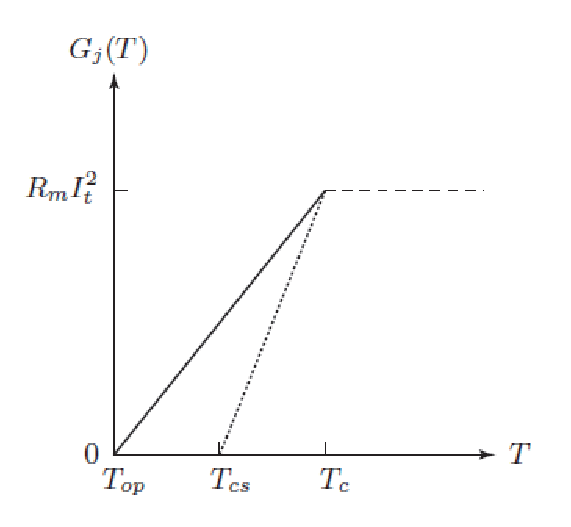
\includegraphics[scale=0.6]{chpt6/figs/fig6.7.eps}
	\caption{复合导体的$G_j(T)$图,其中$R_m$为常数。}
\end{figure}

c) 明显,只要$I_t<I_c(T)$,所有的传输电流都只通过超导体,$V_{cd}=0$,故$G_j(T)=0$。
在电流分享温度$T_{cs}$下,当$I_t=I_c$时,超导体载有其为超导态下的最大可能电流;在$T_{cs}$之上,
电流开始向铜基底分流,在复合导体内产生焦耳热。
随着$T$升高,这个分流持续增加,直到达到$T_c$,在这个点几乎全部传输电流都被转移至基底中,
当然其假设是$R_m\ll R_n$,而它通常是合理的。因为$R_m$是常数,所以$G_j$在温度$T_{cs}$和$T_c$
之间随$T$的变化时线性的。$R_m$是常数这个假设对多数基底金属(如铜)在$T_{op}$小于30 K时都是有效的。

d) 如果$T_{op}>\sim 30$ K,$R_m$的常数假设就不合理的。也即,对多数HTS,应将其做温度依赖看待。
方程6.13b和6.13c相应的修正为:
\begin{subequations}
	\begin{align}
	T_{cs}\leq T\leq T_c:\quad G_j(T)&=R_m(T)I_t^2(\frac{T-T_{cs}}{T_c-T_{cs}})\\
	T\ge T_c:\quad G_j(T)&=R_m(T)I_t^2
	\end{align}
\end{subequations}


\subsection{讨论6.2:Stekly低温稳定性判据}
在6.2.1节,我们看到所谓的Stekly低温稳定性判据通过浸泡到绕组中去的制冷剂平衡了复合超导体产生的焦耳热。
这样,方程6.1可以化简为:
\begin{equation}% page365 第1个 6.15
C_{cd}(T)\frac {\partial T}{\partial t}=\nabla\cdot[k_{cd}(T)\nabla T]+\rho _{cd}(T)J_{cd}^2(t)+g_d(t)-(\frac{f_p\ \mathrm{P}_D}{A_{cd}})g_q(T)
\end{equation}
式中,等号左侧、等号右侧第一项、第三项可以忽略。
式中,$P_D$是从的导体周长;常数$f_D$是置于制冷剂中的$P_D$分数。
Stekly首先通过选择$I_t=I_{c_o}$(令$I_t$等于超导体在$T_{op}$下的临界电流)发展了他的理论。
注意到,$I_t$还表示运行电流$I_{op}$,那么选择$I_t=I_{op}=I_{c_o}$使得$T_{cs}=T_{op}$,
以及6.13b成为:
\begin{subequations}
	\begin{align}
	G_j(T)&=R_mI_{c_o}^2(\frac{T-T_{op}}{T_c-T_{op}}) &(T_{o_p}\leq T \leq T_c)\\
	\rho_{cd}J^2_{cd}(t)&=\frac{\rho_{m}I_{co}^2}{A_{cd}A_m}
	(\frac{T-T_{op}}{T_c-T_{op}}) &(T_{o_p}\leq T \leq T_c)
	\end{align}
\end{subequations}
历史上,Stekly选择$I_t=I_{c_o}$发展他的判据不是为了超导磁体的稳定性,而是为了解释
在V-I测试时超导体测试样品在其电流超过$I_{c_o}$后的分流。
现在,每一个LTS超导磁体的运行电流都选在小于$I_{c_o}$。对于HTS磁体,稳定性不是重要的设计问题;
但是类似LTS测试样品,HTS测试样品也存在稳定性问题。
V-I特性相关的稳定性问题将在问题6.5中研究。

Stekly的冷却选择是温度线性的:
\begin{equation}% page365 第3个 6.17
g_q(T)=h_q(T-T_b)\simeq h_q(T-T_{op})
\end{equation}
式中,$T$是导体的表面问题。$T_b$是冷池(制冷剂)的问题,假定其等于$T_{op}:T_b\simeq T_{op}$。

根据6.15,Stekly低温稳定性判据要求$(f_p P_D/A_{cd})g_q(T)\ge \rho_{cd}(T)J_{cd}^2(t)$。
根据6.16b和6.17,我们有:
\begin{equation*}% page365 第4个 6.18
\frac{f_pP_Dh_q(T-T_{op}}{A_cd}\geq \frac{\rho_m I_{co}^2}{A_{cd}A_m}(\frac{T-T_{op}}{T_c-T_{op}})
\end{equation*}
\begin{equation}% page365 第4个 6.18
\frac{\rho_m I_{co}^2}{f_pP_DA_mh_q(T_c-T_{op})}\leq 1
\end{equation}
Stekly稳定性参数$\alpha_{sk}$由6.18给出:
\begin{equation}% page365 第5个 6.19
\alpha_{sk}=\frac{\rho_m I_{co}^2}{f_pP_DA_mh_q(T_c-T_{op})}
\end{equation}
注意到,无量纲参数$\alpha_{sk}$表示的是焦耳耗散密度和冷却功率的比值。于是,当$\alpha_{sk}\le 1$
时(冷量足够),运行时稳定的;当$\alpha_{sk}> 1$时(冷量不够)不稳定。

根据Stekly稳定性判据,1960年代和1970年代建造和可靠运行的多数大型磁体都是低温稳定的。
方程6.19表明$\alpha_{sk}\propto 1/A_m$,即对给定的冷却条件,稳定性或可靠性与$A_m$有直接关系。反过来:
\begin{equation}% page366 第1个 6.20
A_m=\frac {\rho_mI_{co}^2}{\alpha_{sk}f_pP_Dh_q(T_c-T_{op})}
\end{equation}
为了在给定冷却条件下实现更大程度的稳定性,在浸泡冷却的低温稳定磁体中,增加$A_m$十分必要。
复合超导体在运行电流下的电流密度$J_{op}$为:
\begin{align*}% page366 第2个 6.6
J_{op}=\frac{I_{op}}{A_{sc}+A_ {\bar{m}}+A_m}\tag{6.6}
\end{align*}
\begin{equation}% page366 第2个 6.21a
=(\frac{\gamma_{m/s}}{\gamma_{m/s}+1})J_{m_0}
\end{equation}
式中的面积比$\gamma_{m/s}$定义为:
\begin{align*}% page366 第3个 6.21b
\gamma_{m/s}\equiv \frac{A_m}{A_{sc}+A_m}
\end{align*}
在NbTi中,$\gamma_{m/s}$被称为基底-超导体比率,在$\mathrm{Nb_3Sn}$中称为基底-非基底比率。
显然,当$\gamma_{m/s}\gg 1$时,有$J_{op}\simeq J_m$。

很明显,在这些早期的大型磁体中,稳定性无疑是优先于效率考虑的。这种哲学一直持续到今天,
特别大型磁体。而大型磁体中,还有另一个可能比稳定性更重要的问题需要考虑:电磁力。
大型低温稳定LTS磁体要求的加强组件$A_S$在限制绕组的总电流密度上,比基底金属$A_m$更重要。

表6.5列出了两个低温稳定LTS磁体(一个是1960年代末期的NbTi磁体,一个是近期的CIC $\mathrm{Nb_3Sn}$磁体)的电流参数---$I_c,I_{op},\gamma_{m/s},J_c(=I_c/A_{sc}),J_e(=I_c/A_{cd}),
J_{m_o}(=I_{op}/A_m),\lambda J_{op}(=I_{op}/A_{wd})$[6.12,3.24]。
相比于NbTi磁体,$\mathrm{Nb_3Sn}$磁体的$\gamma_{m/s}$更小,这意味着它的$\lambda J_{op}$更好。
这个性能的提高部分是由于近四十年来随着建造实际磁体而逐步深入的对稳定性和保护问题的理解,
部分来自降低这种仅用于研究的个性化磁体的费用的压力。

表6.5.。。。。。。。。。

\subsection{讨论6.3:复合物超导体}
可用的磁体级超导体通常有两类,一类是“Monolithic”(单体),一类是“built-up”(组合)。

\textbf{A. Monolith}

超导体和正常金属通过简单合金工艺形成一个实体。视觉上看,除了在导体截面上,不能分辨出一个一个单体上存在
多与一种组分。多数圆线复合导体都是单体的。尽管$\gamma_{m/s}$值大于10,但在合金过程中不折断
细丝而生成单体超导体很难,特别是那些细丝直径小于100 $\mu$m的尤其难。

\textbf{B. Build-up}

组合的超导体由$\gamma_{m/s}$接近1的单体超导体和正常金属稳定部分组成,金属稳定部分通常是焊在
处理后的单体上的。稳定部分的机械性能因而不受到单体处理过程的影响,从而能更容易满足导体规格要求。
CIC导体是一种组合导体变种。

\subsection{问题6.2:低温稳定性——非线性冷却曲线}
讨论6.2推出的参数$\alpha_{sk}$是基于与温度无关的传热系数$h_q$的。
实际中,冷却曲线,甚至低温稳定磁体通畅运行的核态沸腾传热区域都是非线性很严重的,一个例子如图4.1所示。
于是,直接从低温稳定性判据导出热流曲线$q(T)[\mathrm{W/cm^2\ or\ W/m^2}] $。

a) 证明$I_{op}$下的基底电流密度$[J_{m_o}]_{sk}$满足Stekly低温稳定性判据的一个变体,
该变体结合了热流密度曲线$q(T)$:
\begin{equation}% page367 第1个 6.22
[J_{m_o}]_{sk}=\sqrt{\frac{f_pP_Dq_{fm}}{\rho_mA_m}}
\end{equation}
式中,$q_{fm}$是膜态沸腾区域的最小热流密度。

b) 在$I_{op}=I_{c_o}$时,在同一个图中定性画出$q(T)$曲线和尺度一致的产热曲线,并在图中指出稳定运行的区域。
其中,$I_{c_o}$是超导体在$T_{op}$时的$I_c$。

c) 在b)的同一个图上推广b)到$I_{op}<I_{c_o}$的情况。证明,在这个条件下,电流分享温区的
$g_j(T_c)$和$d\hat{g}_j(T)/dT$小于$I_{op}=I_{c_o}$条件下的。

\subsubsection{问题6.2之解}
a) 在应用低温稳定性的多数应用中,我们必须假定超导体可能运行在完全正常态。然后,选择膜态沸腾区域的最小热流
是最安全的。于是:
\begin{align*}% page368 第1个 S2.1
\frac {\rho_mI_{co}^2}{A_m}=f_pP_Dq_{fm} \tag{S2.1}
\end{align*}
解出$[J_{m_o}]_{sk}$,得到:
\begin{align*}% page368 第2个 6.22
[J_{m_o}]_{sk}=\sqrt{\frac{f_pP_Dq_{fm}}{\rho_mA_m}} \tag{6.22}
\end{align*}

b) 图6.8给出了液氦$q(T)$的典型曲线。图中同时还画出了$\hat{g}_j(T)\equiv (A_{cd}/f_p P_D)g_j(T)$曲线。
通过选择合适的参数,$\hat{g}_j(T)\equiv (A_{cd}/f_p P_D)g_j(T)$略小于$q_{fm}$。

c) 图6.8中的虚线表示$I_t<I_{c_o}$的情况。在温区$T_{op}\le T\le T_{cs}$,导体是全超导的。
因为$G_j(T_{op})=R_m I_t^2$,很明显,它在$I_t<I_{c_o}$时更小。根据问题6.2的S1.2:
\begin{align*}% page368 第3个 s1.2
I_{c_o}=I_t(\frac{T_c-T_{op} }{T_c-T_{cs}}) \tag{S1.2}
\end{align*}
联立S1.2和6.13b,有:
\begin{align*}% page368 第4个
g_j(T)&=(\frac{A_{cd}}{f_pP_D})R_mI_t^2=(\frac{A_{cd}}{f_pP_D})R_mI_{co}^2\frac{(T_c-T_{cs})^2(T-T_{cs})}{(T_c-T_{op})^3}\\
\frac{dg_j(T)}{dT}&=(\frac{A_{cd}}{f_pP_D})R_mI_{co}^2\frac{(T_c-T_{cs})^2}{(T_c-T_{op})^3}
\end{align*}
这样,$G_j(T_{op})$在$I_t=I_{c_o}(T_{cs}=T_{op})$时就要大于$I_t<I_{c_o}(T_{cs}>T_{op})$对应的值了。
\begin{figure}[htbp]
	\centering
	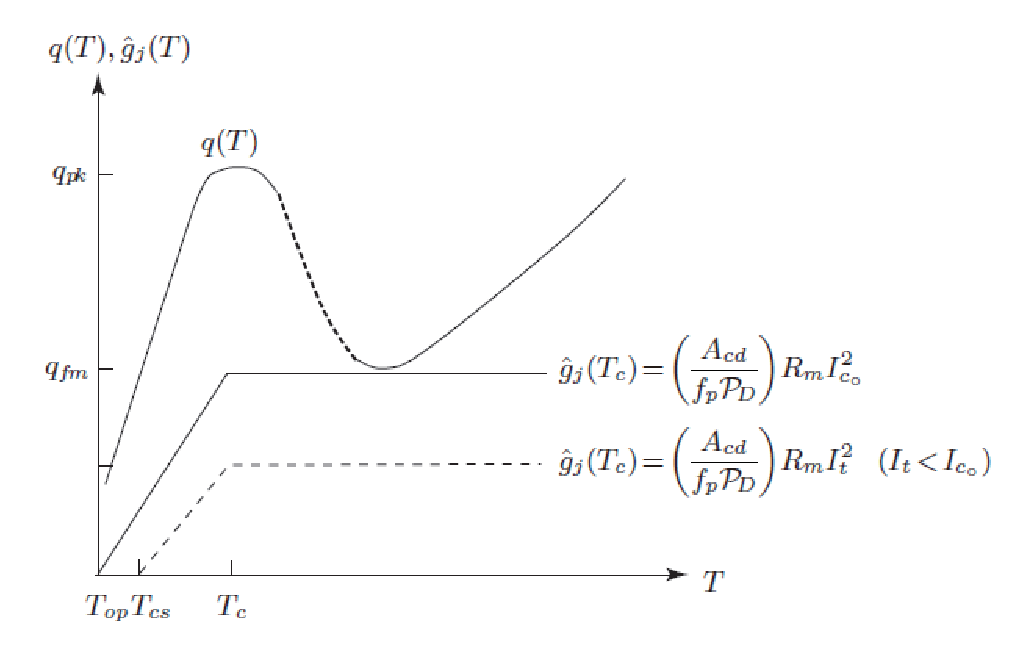
\includegraphics[scale=0.6]{chpt6/figs/fig6.8.eps}
	\caption{液氦$q(T)$的定性图,以及$I_{op}=I_{c_o}$(实线)和$I_{op}<I_{c_o}$(虚线)$两种情况下的$$\hat{g}_j(T)$图。}
\end{figure}


\subsection{讨论6.4:“等面积”判据}
\begin{equation}% page369 第1个 6.23
\int_{T_{op}}^{T_{eq}}[g_q(T)-(\frac{A_{cd}}{f_pP_D})g_j(T)]d(T)
=\int_{T_{op}}^{T_{eq}}[g_q(T)-\hat{g}_j(T)]dT=0
\end{equation}
\begin{equation}% page369 第2个 6.24a
g_j(T)=\rho_m(T)J_{m_o}^2(\frac{T-T_{op}}{T_c-T_{op}}) (T_{op}\leq T \leq T_c)
\end{equation}
\begin{equation}% page369 第3个 6.24b
g_j(T)=\rho_m(T)J_{m_o}^2 (T \geq T_c)
\end{equation}


\subsection{讨论6.5:超导体“指数”n}
\begin{equation}% page370 第1个 6.25a
V_s=V_c(\frac{I_s}{I_c})^n
\end{equation}
\begin{equation}% page370 第2个 6.25b
E_s=E_c(\frac{I_s}{I_c})^n
\end{equation}



\subsection{问题6.3:复合物超导体(n)——电路模型}
\begin{equation}% page371 第1个 6.26a
R_s=R_c(\frac{I_s}{I_c})^{(n-1)}
\end{equation}
\begin{equation}% page371 第2个 6.26b
R_{dif}=nR_c(\frac{I_s}{I_c})^{(n-1)}
\end{equation}

\subsubsection{问题6.3之解}

\begin{equation}% page372 第1个 S3.1
R_s=\frac{V_s}{I_s}=\frac{V_c}{I_s}(\frac{I_s}{I_c})^2=\frac{V_c}{I_c}(\frac{I_s}{I_c})^{(n-1)}
\end{equation}
\begin{equation}% page372 第2个 6.26a
R_s=R_c(\frac{I_s}{I_c})^{(n-1)}
\end{equation}
\begin{equation}% page372 第3个 S3.2
R_{dif}=\frac{\partial V_s}{\partial I_s}=\frac{nV_c}{I_c}(\frac{I_s}{I_c})^{(n-1)}
\end{equation}
\begin{equation}% page372 第4个 6.26a
R_{dif}=nR_c(\frac{I_s}{I_c})^{(n-1)}
\end{equation}
\begin{equation}% page372 第5个S3.3a
I_t=I_m+I_s
\end{equation}
\begin{equation}% page372 第6个S3.3b
V_m=R_mI_m=V_s=V_c(\frac{I_s}{I_c})^{n}
\end{equation}
\begin{equation}% page372 第6个S3.3c
3\times 10^{-4}\ \mathrm{\Omega}\times I_m[\ \mathrm{A}]=10^{-5}V(\frac{90\ \mathrm{A}-I_m[\ \mathrm{A}]}{100\ \mathrm{A}})^{15}
\end{equation}
\begin{equation}% page372 第7个S3.4
P_{cd}=R_mI_mI_t=V_sI_t
\end{equation}



\subsection{问题6.4:电流脉冲下的YBCO}
\begin{equation}% page375 第1个6.27a
R_m(T)=0.190+1.530(\frac{T-77}{293-77})\ [\ \mathrm{m\Omega}]
\end{equation}
\begin{equation}% page375 第1个6.27b
I_c(T)=100(\frac{93-T}{93-77})[\ \mathrm{A}]
\end{equation}
\begin{equation}% page375 第1个6.27C
V_s(T)=5[\frac{I_s(T)}{I_c(T)}]^{10} [\ \mathrm{\mu V}]
\end{equation}


\subsubsection{问题6.4之解}

\begin{equation}% page376 第1个S4.1a
I_t=I_s+I_m
\end{equation}
\begin{equation}% page376 第2个S4.1b
R_mI_m=V_s(I_s)
\end{equation}
\begin{equation}% page376 第3个S4.2a
I_s=(290\ \mathrm{A})-I_m
\end{equation}
\begin{equation}% page376 第4个S4.2b
(0.19\times10^{-3}\ \mathrm{\Omega})I_m=(5\times10^{-6}\ \mathrm{V})(\frac{290\ \mathrm {A}-I_m}{100\ \mathrm{A}})^{10}
\end{equation}
\begin{equation}% page376 第5个S4.3
(18\times10^{-3}\ \mathrm{V})=(5\times10^{-6}\ \mathrm{V})(\frac{195.26\ \mathrm{A}}{100\ \mathrm{A}})^n
\end{equation}
\begin{equation}% page376 第6个S4.4
V_{cd}=40\times10^{-3}\ \mathrm{V}=R_m(T)I_m
\end{equation}
\begin{equation}% page376 第7个S4.5a
10\times10^{-3}=[{[0.190+1.530(\frac{T-77}{293-77})]^\times10^{-3}\ \mathrm{\Omega}}]I_m(T)
\end{equation}
\begin{equation}% page376 第8个S4 .5b I_m(T)=\frac{40\times10^{-3}\ \mathrm{V}}{[0.190+1.530(\frac{T-77}{293-77})]\times10^{-3}\ \mathrm{\Omega}}I_m(T)
\end{equation}
\begin{equation}% page376 第9个S4 .5c
=\frac{40}{0.190+1.530(\frac{T-77}{293-77})}\ \mathrm{A}
\end{equation}
\begin{equation}% page377 第1个S4.6
40\times10^{-3}\ \mathrm{V}=(5\times10^{-6}V)[\frac{300A-I_m(T)}{I_c(T)}]^{12.24}
\end{equation}
\begin{equation}% page377 第2个S4.7
40\times10^{-3}\ \mathrm{V}=(5\times10^{-6}V)[\frac{300\ \mathrm{A}-\frac{40\ \mathrm{A}}{[0.190+1.530(\frac{T-77}{293-77})]}}{(100\ \mathrm{A})(\frac{93-T}{93-77})}]^{12.24}
\end{equation}
\begin{equation}% page377 第3个S4.8
8000=[\frac{16(406200T-28027799)}{(93-T)(135400T-6793895)}]^{12.24}
\end{equation}


\subsection{讨论6.6:CICC导体}
\begin{equation}% page378 第1个6.28a
C_{cd}(T)\frac{\partial T}{\partial t}=\nabla.[k_{cd}(T)\nabla T]+\rho_{cd}(T)J_{cd_o}^2(t)+g_d(t)-(\frac{f_pP_D}{A_{cd}})h_{he}(T-T_{he})
\end{equation}
\begin{equation}% page378 第2个6.28b
C_{he}(T_{he})\frac{\partial T_{he}}{\partial t}=(\frac{f_{p}P_D}{A_cd})h_{he}(T-T_{he})
\end{equation}
\begin{equation}% page379 第1个6.29
h_{he}=0.0259(\frac{k_{he}}{D_{hy}})Re^{0.8}Pr^{0.4}(\frac{T_{he}}{T_{cd}})^{-0.716}
\end{equation}
\begin{equation}% page381 第1个6.30
I_{lim}=\sqrt{\frac{A_mf_p\ \mathrm{P}_Dh_{he}(T_c-T_{op})}{\rho_m}}
\end{equation}




\subsection{问题6.5:冷却复合物导体的伏安关系}


\begin{equation}% page383 第1个6.31
V=\frac{R_m(I-I_{co})}{1-\frac{R_mII_{co}}{f_pP_{cd}\ell h_q(T_c-T_{op})}}
\end{equation}
\begin{equation}% page383 第2个6.32
\ \mathrm{u}(\ \mathrm{i})=\frac{\ \mathrm{i}-1}{1-\alpha_{ski}}
\end{equation}


\subsubsection{问题6.5之解}
\begin{equation}% page384 第1个S5.1
G_{j}(T_{op}+\triangle T)=VI=R_m\{I-I_{co}[\frac{T_c-(T_{op}+\Delta T)}{T_c-T_{op}}]\}I
\end{equation}
\begin{equation}% page384 第1个S5.1
=R_mI[(I-I_{co})+\frac{I_{co}\Delta T}{T_c-T_{op}}]
\end{equation}
\begin{equation}% page384 第2个S52
\Delta T=\frac{R_mI(I-I_{c_o})(T-T_{op})}{f_pP_{cd}\ell h_q(T_c-T_{op})-R_mI_{c_o}I}
\end{equation}
\begin{equation}% page384 第3个S5.3a
V=R_m\{(I-I_{c_o})+\frac{I_{c_o}}{T_c-T_{op}}[\frac{R_mI(I-I_{co})(T_c-T_{op})}{f_pP_{cd}\ell h_q(T_c-T_{op})-R_mI_{c_o}I}]\}
\end{equation}
\begin{equation}% page384 第4个S5.3b
=R_m(I-I_{c_o}))+\frac{R_m^2I_{c_o}(I-I_(co))}{f_pP_{cd}\ell h_q(T_c-T_{op})-R_mI_{c_o}I}
\end{equation}
\begin{equation}% page384 第5个6.31
V=\frac{R_m(I-I_{co})}{1-\frac{R_mII_{co}}{f_pP_{cd}\ell h_q(T_c-T_{op})}}
\end{equation}
\begin{equation}% page384 第6个
V=\frac{R_m(I-I_{co})}{1-\alpha_{sk}(I/I_{co})}
\end{equation}
\begin{equation}% page384 第7个
v(i)=\frac{i-1}{1-\alpha_{sk}i}
\end{equation}
\begin{equation}% page384 第8个
\alpha_{sk}=\frac{\rho_mI_{co^2}}{f_pP_{cd}A_mh_q(T_c-T_{op})}
\end{equation}
\begin{equation}% page384 第9个
=\frac{(4\times10^{-10}\ \mathrm{\Omega m})(100\ \mathrm{A})^2}{(1)(2\times10^{-2}\ \mathrm{m^2})(10^4\ \mathrm{W/m^2K})(5.2\ \mathrm{K}-4.2\ \mathrm{K})}=0.1
\end{equation}
\begin{equation}% page384 第10个
v(i)=\frac{10(i-1)}{10-i}
\end{equation}


\subsection{问题6.6:混合III SCM的稳定性分析}

\begin{equation}% page387 第1个
q_k=a_k(T^{n_k}_{cd}-T^{n_k}_b)
\end{equation}
\subsubsection{问题6.6之解}



\subsection{讨论6.7:cryostable vs 准绝热磁体}



\subsection{讨论6.8:MPZ概念}



\begin{equation}% page391 第1个
R_{mz}=\sqrt{\frac{3k_{wd}(T_c-T_{op})}{\rho_mJ_m^2}}
\end{equation}



\subsection{问题6.7:绝热绕组中的耗散能密度}

\begin{equation}% page392 第1个
0=\nabla.[k_{wd}(T)\nabla T]+g_d(t)
\end{equation}
\begin{equation}% page392 第2个
T(\rho)=\frac{a_1^2gd}{4k_{wd}}[(1-\rho^2)+(\frac{\alpha^2-1}{\ln \alpha})\ln\rho]+T_{op}
\end{equation}
\begin{equation}% page392 第3个
\rho_{mx}=\sqrt{\frac{\alpha^2-1}{2\ln \alpha}}
\end{equation}
\begin{equation}% page392 第4个
g_{d_c}=\frac{4k_{wd}\Delta T_{mx}}{a_1^2\{1+\frac{\alpha^2-1}{2\ln \alpha}[\ln{(\frac{\alpha^2-1}{2\ln\alpha})}-1]\}}
\end{equation}
\begin{equation}% page392 第5个
g_{dc}=(\frac{k_{wd}\Delta T_{mx}}{a_1^2})\gamma_{d_c}(\alpha)
\end{equation}
\begin{equation}% page392 第6个
\gamma_{d_c}(\alpha)\equiv\frac{4}{1+\frac{\alpha-1}{2\ln\alpha}[\ln(\frac{\alpha^2-1}{2\ln\alpha})-1]}
\end{equation}


\subsubsection{问题6.7之解}
\begin{equation}% page393 第1个
\frac{k_{wd}}{r} \frac{d}{dr}(r\frac{dT}{dr})+g_d=0
\end{equation}
\begin{equation}% page393 第2个
\frac{k_{wd}}{\rho}\frac{d}{d\rho}(\rho\frac{dT}{d\rho})+g_da_1^2=0
\end{equation}
\begin{equation}% page393 第3个
T(\rho)=-\frac{g_da_1^2}{4k_{wd}}\rho^2+A\ln\rho+B
\end{equation}
\begin{equation}% page393 第4个
T(\rho)=-\frac{g_da_1^2}{4k_{wd}}[(1-\rho^2)+(\frac{\alpha-1}{\ln\alpha})\ln\rho]+T_{op}
\end{equation}
\begin{equation}% page393 第5个
\frac{dT}{d\rho}=\frac{g_da_1^2}{4k_{wd}}[-2\rho+(\frac{\alpha^2-1}{\ln\alpha})\frac{1}{\rho}]=0
\end{equation}
\begin{equation}% page393 第6个
\rho_{mx}=\sqrt{\frac{\alpha^2-1}{2\ln\alpha}}
\end{equation}
\begin{equation}% page393 第7个
T(\rho_{mx})\equiv T_{mx}=\frac{a_1^2g_d}{4k_{wd}}[(1-\rho_{mx}^2)+(\frac{\alpha^2-1}{\ln\alpha})\ln\rho_{mx}]+T_{op}
\end{equation}
\begin{equation}% page393 第8个
\Delta T_{mx}=\frac{g_{d_c}a_1^2}{4k_{wd}}(1+\frac{\alpha^2-1}{2\ln\alpha}[\ln(\frac{\alpha^2-1}{2\ln\alpha})-1])
\end{equation}
\begin{equation}% page393 第9个
g_{d_c}=\frac{4k_{wd}\Delta T_{mx}}{a_1^2\{(1+\frac{\alpha^2-1}{2\ln\alpha}[\ln(\frac{\alpha^2-1}{2\ln\alpha})-)\}}
\end{equation}
\begin{equation}% page394 第1个
g_{d_c}=(\frac{k_{wd}\Delta T_{mx}}{a_1^2})\gamma_{d_c}(\alpha)
\end{equation}
\begin{equation}% page394 第1个
=\frac{(0.01\ \mathrm{W/cmK})(3\ \mathrm{K})}{(10\ \mathrm{cm})^2}(7.9)\simeq2.4\times10^{-3}\ \mathrm{W/cm^3}\simeq2.4\times10^3\ \mathrm{W/m^3}
\end{equation}


